\section{Kant finder}
\subsection{Verificering og validering}
Vi kan køre billeder igennem vores kant-finde og derved se om billedernes kanter stemmer overens.
Dette kan give en ide om hvor god vores kant-finder er.
Se billeder:
\begin{figure}
\centering
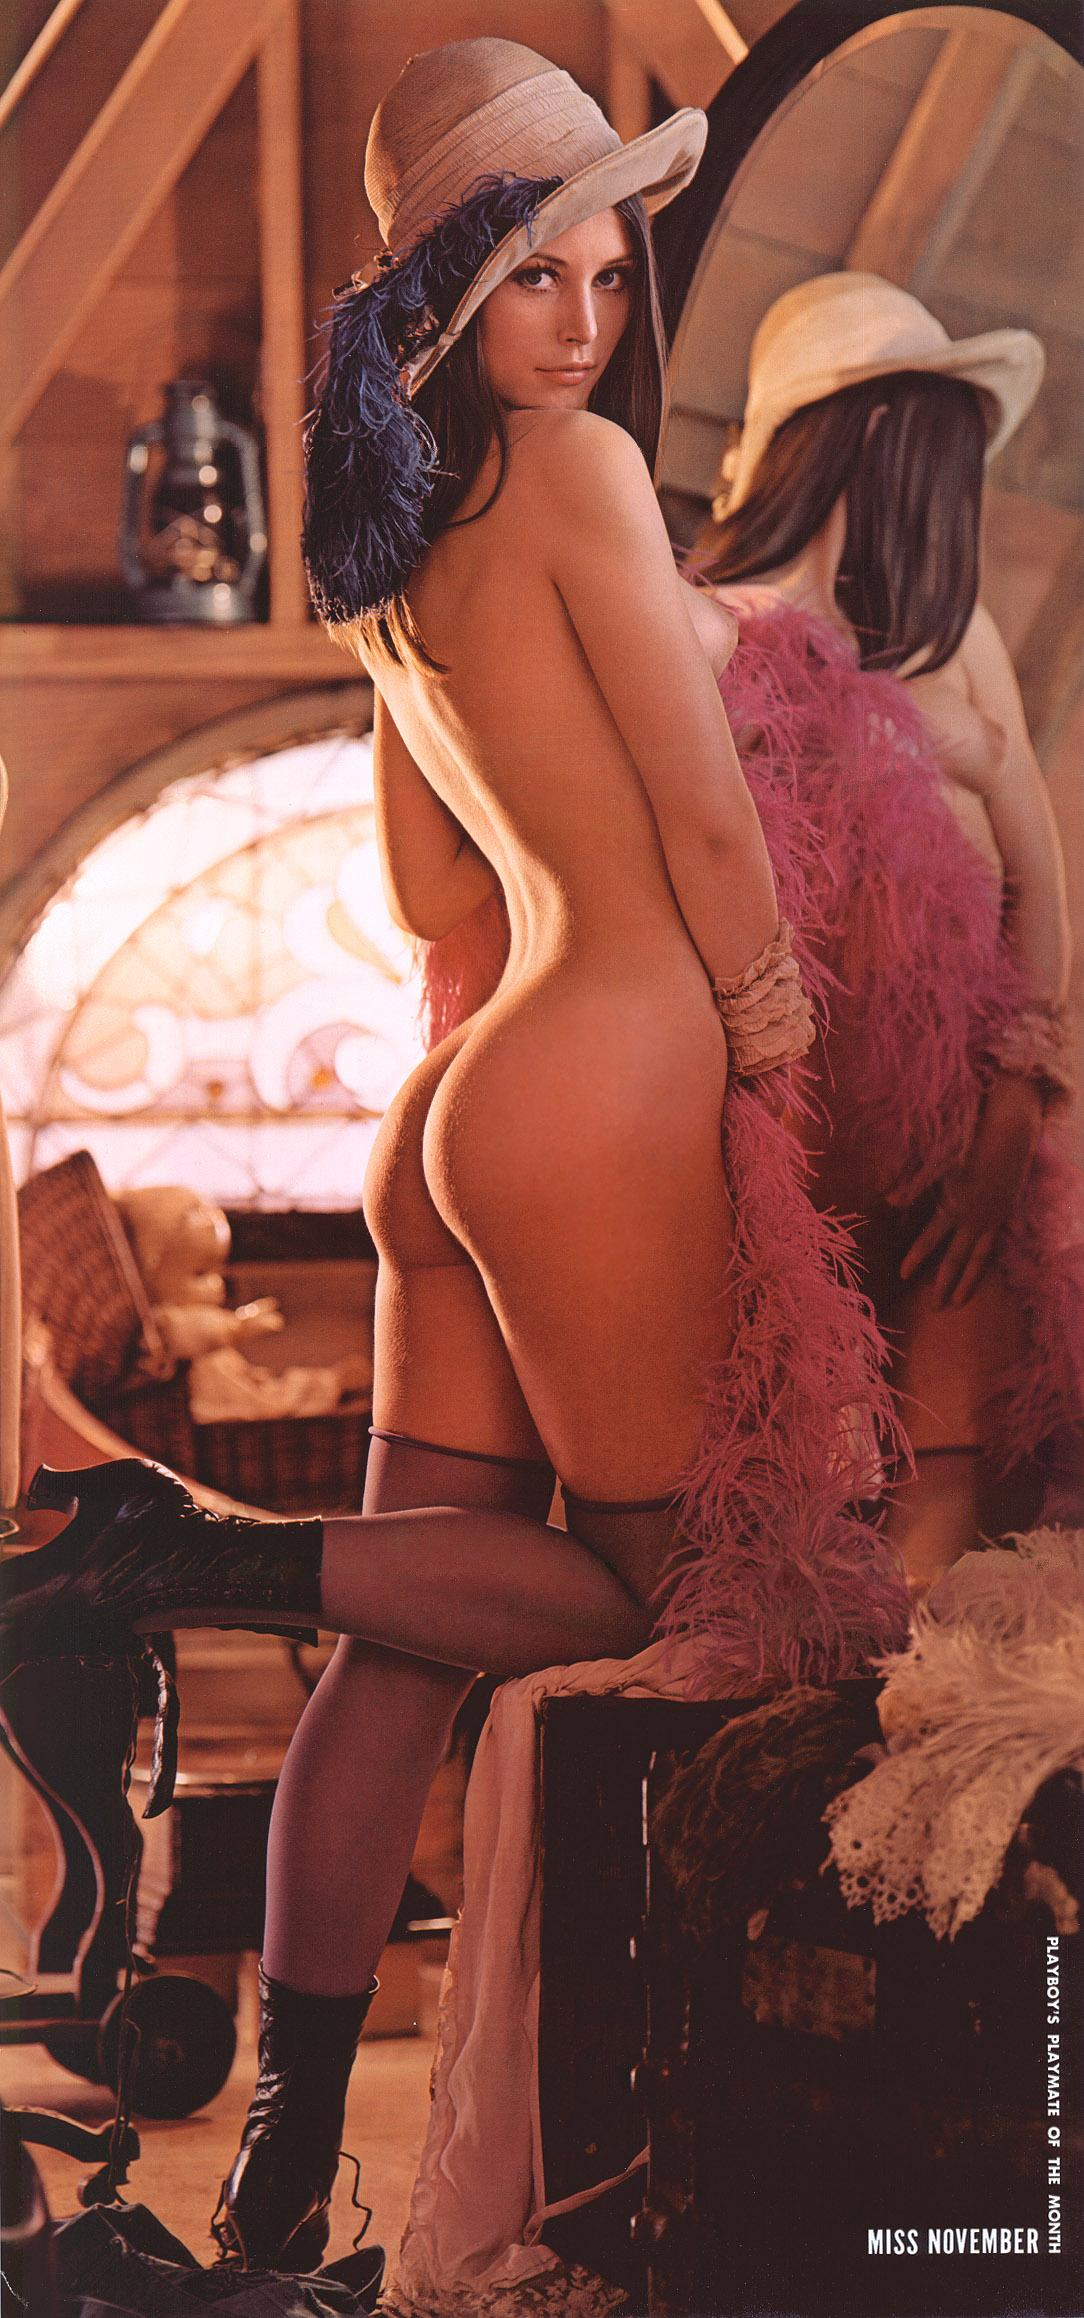
\includegraphics[scale=0.3]{lena}
\caption{Originalt lena billed}
\end{figure}
\begin{figure}
\centering
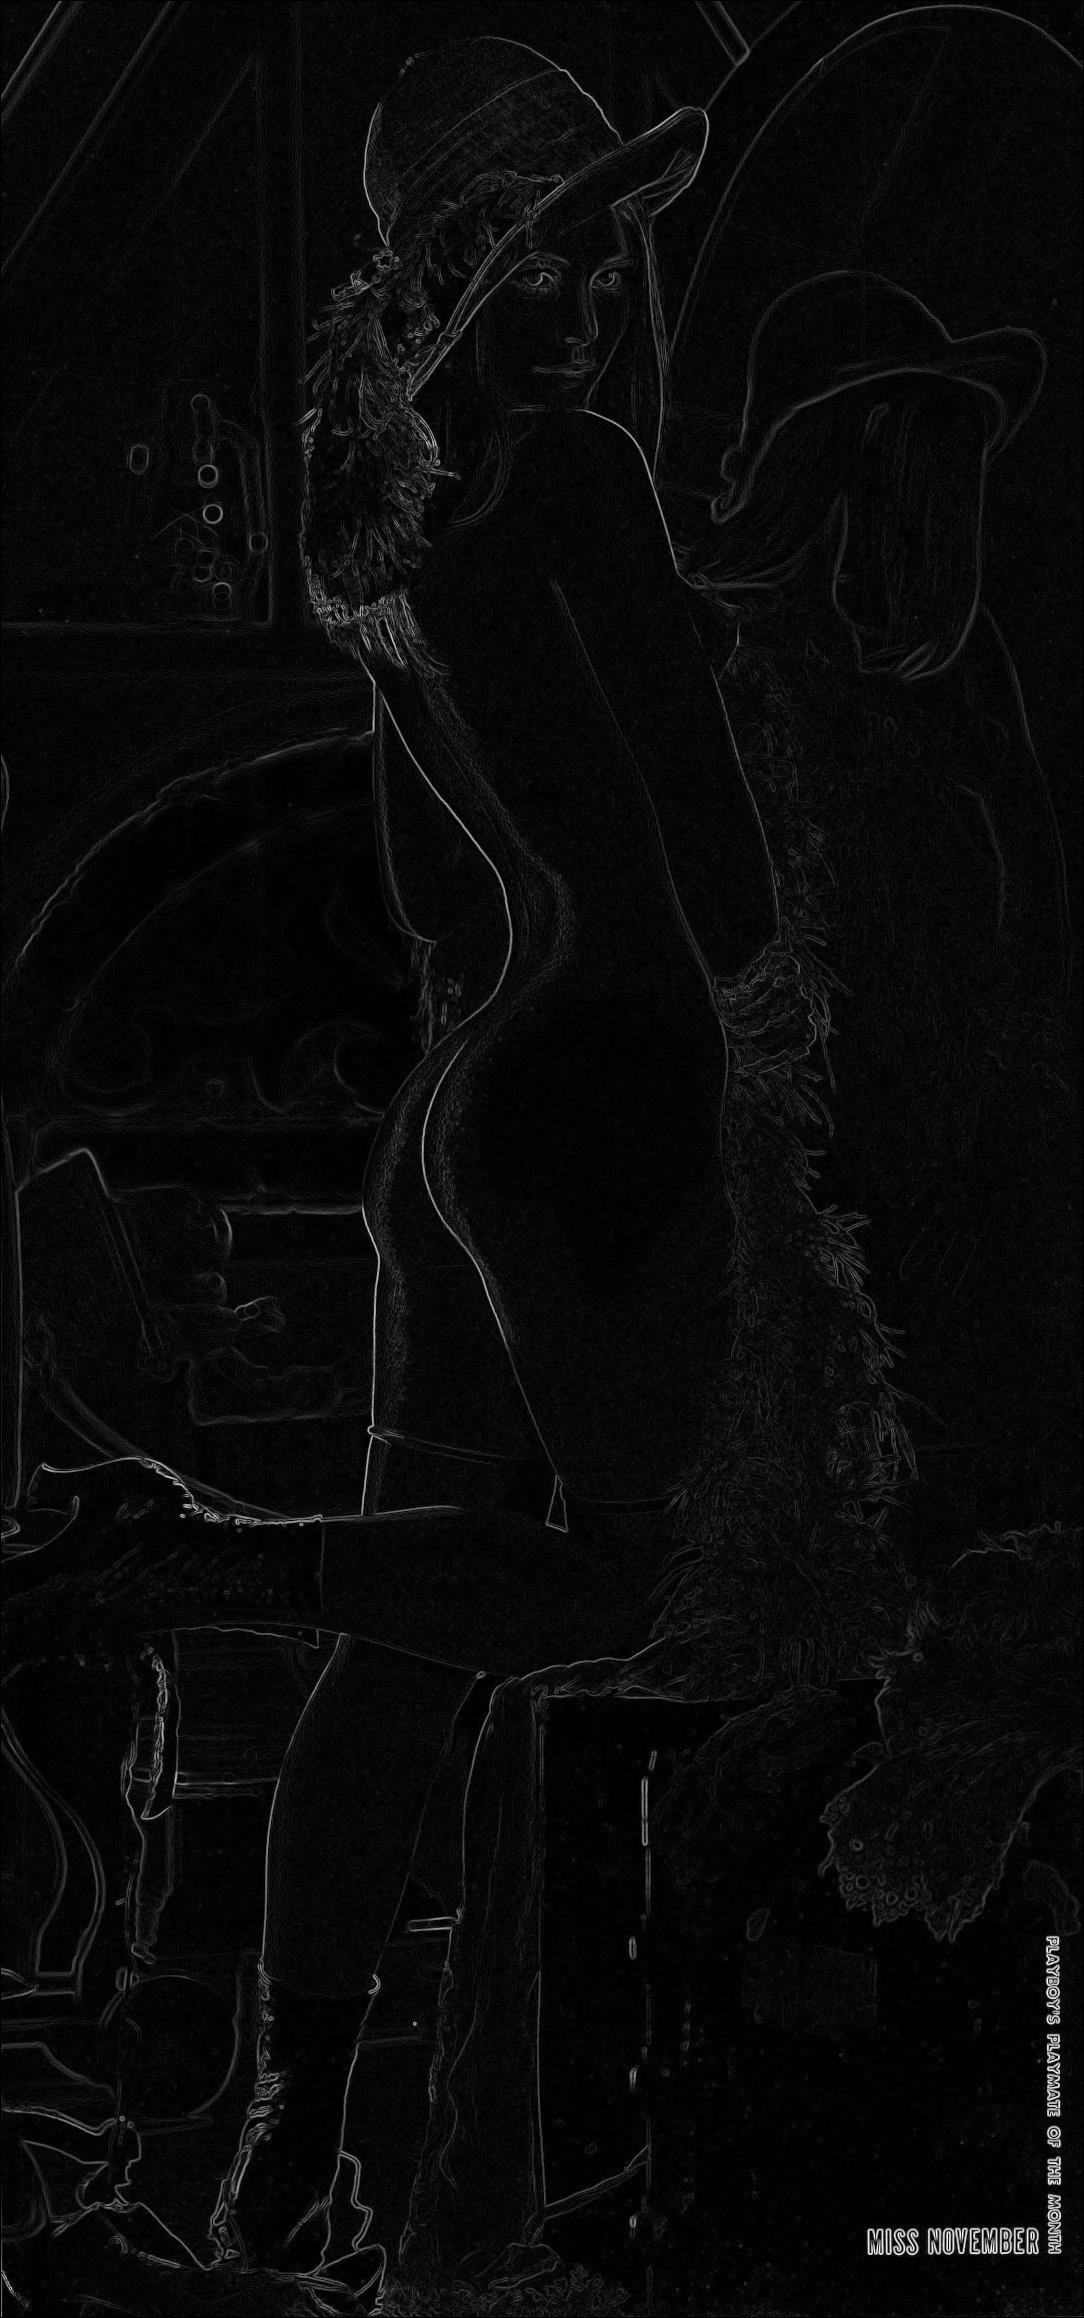
\includegraphics[scale=0.25]{lena_edges}
\caption{Lena billed efter kant finder funktionen}
\end{figure}
\begin{figure}
\centering

\includegraphics{Donkey-kong}
\caption{Originalt Donkey Kong billed}
\end{figure}
\begin{figure}
\centering
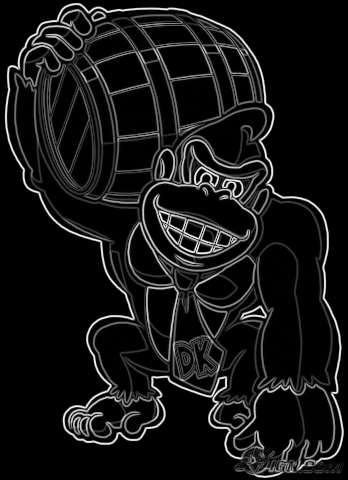
\includegraphics{Donkey-kong_edges}
\caption{Donkey Kong billed efter kant finder funktionen}
\end{figure}

